% Options for packages loaded elsewhere
\PassOptionsToPackage{unicode}{hyperref}
\PassOptionsToPackage{hyphens}{url}
\PassOptionsToPackage{dvipsnames,svgnames,x11names}{xcolor}
%
\documentclass[
  letterpaper,
  DIV=11,
  numbers=noendperiod]{scrartcl}

\usepackage{amsmath,amssymb}
\usepackage{iftex}
\ifPDFTeX
  \usepackage[T1]{fontenc}
  \usepackage[utf8]{inputenc}
  \usepackage{textcomp} % provide euro and other symbols
\else % if luatex or xetex
  \usepackage{unicode-math}
  \defaultfontfeatures{Scale=MatchLowercase}
  \defaultfontfeatures[\rmfamily]{Ligatures=TeX,Scale=1}
\fi
\usepackage{lmodern}
\ifPDFTeX\else  
    % xetex/luatex font selection
\fi
% Use upquote if available, for straight quotes in verbatim environments
\IfFileExists{upquote.sty}{\usepackage{upquote}}{}
\IfFileExists{microtype.sty}{% use microtype if available
  \usepackage[]{microtype}
  \UseMicrotypeSet[protrusion]{basicmath} % disable protrusion for tt fonts
}{}
\makeatletter
\@ifundefined{KOMAClassName}{% if non-KOMA class
  \IfFileExists{parskip.sty}{%
    \usepackage{parskip}
  }{% else
    \setlength{\parindent}{0pt}
    \setlength{\parskip}{6pt plus 2pt minus 1pt}}
}{% if KOMA class
  \KOMAoptions{parskip=half}}
\makeatother
\usepackage{xcolor}
\setlength{\emergencystretch}{3em} % prevent overfull lines
\setcounter{secnumdepth}{-\maxdimen} % remove section numbering
% Make \paragraph and \subparagraph free-standing
\ifx\paragraph\undefined\else
  \let\oldparagraph\paragraph
  \renewcommand{\paragraph}[1]{\oldparagraph{#1}\mbox{}}
\fi
\ifx\subparagraph\undefined\else
  \let\oldsubparagraph\subparagraph
  \renewcommand{\subparagraph}[1]{\oldsubparagraph{#1}\mbox{}}
\fi

\usepackage{color}
\usepackage{fancyvrb}
\newcommand{\VerbBar}{|}
\newcommand{\VERB}{\Verb[commandchars=\\\{\}]}
\DefineVerbatimEnvironment{Highlighting}{Verbatim}{commandchars=\\\{\}}
% Add ',fontsize=\small' for more characters per line
\usepackage{framed}
\definecolor{shadecolor}{RGB}{241,243,245}
\newenvironment{Shaded}{\begin{snugshade}}{\end{snugshade}}
\newcommand{\AlertTok}[1]{\textcolor[rgb]{0.68,0.00,0.00}{#1}}
\newcommand{\AnnotationTok}[1]{\textcolor[rgb]{0.37,0.37,0.37}{#1}}
\newcommand{\AttributeTok}[1]{\textcolor[rgb]{0.40,0.45,0.13}{#1}}
\newcommand{\BaseNTok}[1]{\textcolor[rgb]{0.68,0.00,0.00}{#1}}
\newcommand{\BuiltInTok}[1]{\textcolor[rgb]{0.00,0.23,0.31}{#1}}
\newcommand{\CharTok}[1]{\textcolor[rgb]{0.13,0.47,0.30}{#1}}
\newcommand{\CommentTok}[1]{\textcolor[rgb]{0.37,0.37,0.37}{#1}}
\newcommand{\CommentVarTok}[1]{\textcolor[rgb]{0.37,0.37,0.37}{\textit{#1}}}
\newcommand{\ConstantTok}[1]{\textcolor[rgb]{0.56,0.35,0.01}{#1}}
\newcommand{\ControlFlowTok}[1]{\textcolor[rgb]{0.00,0.23,0.31}{#1}}
\newcommand{\DataTypeTok}[1]{\textcolor[rgb]{0.68,0.00,0.00}{#1}}
\newcommand{\DecValTok}[1]{\textcolor[rgb]{0.68,0.00,0.00}{#1}}
\newcommand{\DocumentationTok}[1]{\textcolor[rgb]{0.37,0.37,0.37}{\textit{#1}}}
\newcommand{\ErrorTok}[1]{\textcolor[rgb]{0.68,0.00,0.00}{#1}}
\newcommand{\ExtensionTok}[1]{\textcolor[rgb]{0.00,0.23,0.31}{#1}}
\newcommand{\FloatTok}[1]{\textcolor[rgb]{0.68,0.00,0.00}{#1}}
\newcommand{\FunctionTok}[1]{\textcolor[rgb]{0.28,0.35,0.67}{#1}}
\newcommand{\ImportTok}[1]{\textcolor[rgb]{0.00,0.46,0.62}{#1}}
\newcommand{\InformationTok}[1]{\textcolor[rgb]{0.37,0.37,0.37}{#1}}
\newcommand{\KeywordTok}[1]{\textcolor[rgb]{0.00,0.23,0.31}{#1}}
\newcommand{\NormalTok}[1]{\textcolor[rgb]{0.00,0.23,0.31}{#1}}
\newcommand{\OperatorTok}[1]{\textcolor[rgb]{0.37,0.37,0.37}{#1}}
\newcommand{\OtherTok}[1]{\textcolor[rgb]{0.00,0.23,0.31}{#1}}
\newcommand{\PreprocessorTok}[1]{\textcolor[rgb]{0.68,0.00,0.00}{#1}}
\newcommand{\RegionMarkerTok}[1]{\textcolor[rgb]{0.00,0.23,0.31}{#1}}
\newcommand{\SpecialCharTok}[1]{\textcolor[rgb]{0.37,0.37,0.37}{#1}}
\newcommand{\SpecialStringTok}[1]{\textcolor[rgb]{0.13,0.47,0.30}{#1}}
\newcommand{\StringTok}[1]{\textcolor[rgb]{0.13,0.47,0.30}{#1}}
\newcommand{\VariableTok}[1]{\textcolor[rgb]{0.07,0.07,0.07}{#1}}
\newcommand{\VerbatimStringTok}[1]{\textcolor[rgb]{0.13,0.47,0.30}{#1}}
\newcommand{\WarningTok}[1]{\textcolor[rgb]{0.37,0.37,0.37}{\textit{#1}}}

\providecommand{\tightlist}{%
  \setlength{\itemsep}{0pt}\setlength{\parskip}{0pt}}\usepackage{longtable,booktabs,array}
\usepackage{calc} % for calculating minipage widths
% Correct order of tables after \paragraph or \subparagraph
\usepackage{etoolbox}
\makeatletter
\patchcmd\longtable{\par}{\if@noskipsec\mbox{}\fi\par}{}{}
\makeatother
% Allow footnotes in longtable head/foot
\IfFileExists{footnotehyper.sty}{\usepackage{footnotehyper}}{\usepackage{footnote}}
\makesavenoteenv{longtable}
\usepackage{graphicx}
\makeatletter
\def\maxwidth{\ifdim\Gin@nat@width>\linewidth\linewidth\else\Gin@nat@width\fi}
\def\maxheight{\ifdim\Gin@nat@height>\textheight\textheight\else\Gin@nat@height\fi}
\makeatother
% Scale images if necessary, so that they will not overflow the page
% margins by default, and it is still possible to overwrite the defaults
% using explicit options in \includegraphics[width, height, ...]{}
\setkeys{Gin}{width=\maxwidth,height=\maxheight,keepaspectratio}
% Set default figure placement to htbp
\makeatletter
\def\fps@figure{htbp}
\makeatother

\KOMAoption{captions}{tableheading}
\makeatletter
\makeatother
\makeatletter
\makeatother
\makeatletter
\@ifpackageloaded{caption}{}{\usepackage{caption}}
\AtBeginDocument{%
\ifdefined\contentsname
  \renewcommand*\contentsname{Table of contents}
\else
  \newcommand\contentsname{Table of contents}
\fi
\ifdefined\listfigurename
  \renewcommand*\listfigurename{List of Figures}
\else
  \newcommand\listfigurename{List of Figures}
\fi
\ifdefined\listtablename
  \renewcommand*\listtablename{List of Tables}
\else
  \newcommand\listtablename{List of Tables}
\fi
\ifdefined\figurename
  \renewcommand*\figurename{Figure}
\else
  \newcommand\figurename{Figure}
\fi
\ifdefined\tablename
  \renewcommand*\tablename{Table}
\else
  \newcommand\tablename{Table}
\fi
}
\@ifpackageloaded{float}{}{\usepackage{float}}
\floatstyle{ruled}
\@ifundefined{c@chapter}{\newfloat{codelisting}{h}{lop}}{\newfloat{codelisting}{h}{lop}[chapter]}
\floatname{codelisting}{Listing}
\newcommand*\listoflistings{\listof{codelisting}{List of Listings}}
\makeatother
\makeatletter
\@ifpackageloaded{caption}{}{\usepackage{caption}}
\@ifpackageloaded{subcaption}{}{\usepackage{subcaption}}
\makeatother
\makeatletter
\@ifpackageloaded{tcolorbox}{}{\usepackage[skins,breakable]{tcolorbox}}
\makeatother
\makeatletter
\@ifundefined{shadecolor}{\definecolor{shadecolor}{rgb}{.97, .97, .97}}
\makeatother
\makeatletter
\makeatother
\makeatletter
\makeatother
\ifLuaTeX
  \usepackage{selnolig}  % disable illegal ligatures
\fi
\IfFileExists{bookmark.sty}{\usepackage{bookmark}}{\usepackage{hyperref}}
\IfFileExists{xurl.sty}{\usepackage{xurl}}{} % add URL line breaks if available
\urlstyle{same} % disable monospaced font for URLs
\hypersetup{
  pdftitle={Go Fund Me Data Analysis},
  pdfauthor={Matthew Roohan (mlr287), Aishwarya Gupta (ag2469), Ryun Shim, Helena Xiong},
  colorlinks=true,
  linkcolor={blue},
  filecolor={Maroon},
  citecolor={Blue},
  urlcolor={Blue},
  pdfcreator={LaTeX via pandoc}}

\title{Go Fund Me Data Analysis}
\author{Matthew Roohan (mlr287), Aishwarya Gupta (ag2469), Ryun Shim,
Helena Xiong}
\date{}

\begin{document}
\maketitle
\ifdefined\Shaded\renewenvironment{Shaded}{\begin{tcolorbox}[boxrule=0pt, enhanced, frame hidden, breakable, interior hidden, sharp corners, borderline west={3pt}{0pt}{shadecolor}]}{\end{tcolorbox}}\fi

\hypertarget{data-and-packages}{%
\subsection{Data and packages}\label{data-and-packages}}

We start with loading the packages we'll use.

\begin{Shaded}
\begin{Highlighting}[]
\FunctionTok{library}\NormalTok{(tidyverse)}
\end{Highlighting}
\end{Shaded}

\begin{verbatim}
-- Attaching core tidyverse packages ------------------------ tidyverse 2.0.0 --
v dplyr     1.1.4     v readr     2.1.5
v forcats   1.0.0     v stringr   1.5.1
v ggplot2   3.5.0     v tibble    3.2.1
v lubridate 1.9.3     v tidyr     1.3.1
v purrr     1.0.2     
-- Conflicts ------------------------------------------ tidyverse_conflicts() --
x dplyr::filter() masks stats::filter()
x dplyr::lag()    masks stats::lag()
i Use the conflicted package (<http://conflicted.r-lib.org/>) to force all conflicts to become errors
\end{verbatim}

\begin{Shaded}
\begin{Highlighting}[]
\FunctionTok{library}\NormalTok{(dplyr)}
\FunctionTok{library}\NormalTok{(ggplot2)}
\FunctionTok{library}\NormalTok{(tidytext)}
\FunctionTok{library}\NormalTok{(tm)}
\end{Highlighting}
\end{Shaded}

\begin{verbatim}
Loading required package: NLP

Attaching package: 'NLP'

The following object is masked from 'package:ggplot2':

    annotate
\end{verbatim}

\begin{Shaded}
\begin{Highlighting}[]
\FunctionTok{library}\NormalTok{(SnowballC)}
\FunctionTok{library}\NormalTok{(wordcloud)}
\end{Highlighting}
\end{Shaded}

\begin{verbatim}
Loading required package: RColorBrewer
\end{verbatim}

\begin{Shaded}
\begin{Highlighting}[]
\FunctionTok{library}\NormalTok{(RColorBrewer)}
\FunctionTok{library}\NormalTok{(syuzhet)}
\FunctionTok{library}\NormalTok{(randomForest)}
\end{Highlighting}
\end{Shaded}

\begin{verbatim}
randomForest 4.7-1.1
Type rfNews() to see new features/changes/bug fixes.

Attaching package: 'randomForest'

The following object is masked from 'package:dplyr':

    combine

The following object is masked from 'package:ggplot2':

    margin
\end{verbatim}

\begin{Shaded}
\begin{Highlighting}[]
\FunctionTok{library}\NormalTok{(caTools)}
\FunctionTok{library}\NormalTok{(maps)}
\end{Highlighting}
\end{Shaded}

\begin{verbatim}

Attaching package: 'maps'

The following object is masked from 'package:purrr':

    map
\end{verbatim}

\begin{Shaded}
\begin{Highlighting}[]
\FunctionTok{library}\NormalTok{(scales)}
\end{Highlighting}
\end{Shaded}

\begin{verbatim}

Attaching package: 'scales'

The following object is masked from 'package:syuzhet':

    rescale

The following object is masked from 'package:purrr':

    discard

The following object is masked from 'package:readr':

    col_factor
\end{verbatim}

\begin{Shaded}
\begin{Highlighting}[]
\NormalTok{gfm\_data }\OtherTok{\textless{}{-}} \FunctionTok{read.csv}\NormalTok{(}\StringTok{"data/gfm\_cleaned\_data.csv"}\NormalTok{)}
\end{Highlighting}
\end{Shaded}

\hypertarget{data-analysis-components}{%
\subsection{Data Analysis Components:}\label{data-analysis-components}}

\begin{itemize}
\item
  Fundraising Goals and Donor Engagement

  \begin{itemize}
  \item
    How do different initial fundraising goals impact the number of
    donations received and donor engagement on GoFundMe?''
  \item
    Do campaigns with higher initial fundraising goals tend to receive
    more donations, or do more modest goals attract greater donor
    engagement?
  \item
    To what extent do campaigns with personalized stories or unique
    appeals attract more donors and achieve higher fundraising goals
    compared to campaigns with generic messages?
  \end{itemize}
\item
  Social Media Pattern \& Geographical Pattern

  \begin{itemize}
  \item
    What is the correlation between social media engagement metrics
    (likes, shares, comments) and the amount of funds raised in GoFundMe
    campaigns?''
  \item
    Are there discernible geographic patterns in campaign success on
    GoFundMe? Do campaigns in specific regions or cities tend to achieve
    higher fundraising goals?
  \end{itemize}
\item
  Time analysis:

  \begin{itemize}
  \tightlist
  \item
    How does the length of the fundraising campaign impact its success?
    Are longer or shorter campaigns more effective in reaching their
    funding goals?'
  \end{itemize}
\end{itemize}

\hypertarget{time-analysis}{%
\subsection{Time Analysis:}\label{time-analysis}}

\begin{Shaded}
\begin{Highlighting}[]
\CommentTok{\#was the goal reached or not?}
\NormalTok{gfm\_data}\SpecialCharTok{$}\NormalTok{goal\_reached }\OtherTok{\textless{}{-}} \FunctionTok{ifelse}\NormalTok{(gfm\_data}\SpecialCharTok{$}\NormalTok{amount\_raised }\SpecialCharTok{\textgreater{}=}\NormalTok{gfm\_data}\SpecialCharTok{$}\NormalTok{goal, }\StringTok{"Yes"}\NormalTok{, }\StringTok{"No"}\NormalTok{)}

\CommentTok{\#Creating time analysis dataset }
\NormalTok{time\_analysis }\OtherTok{\textless{}{-}} \FunctionTok{select}\NormalTok{(gfm\_data, category, position, amount\_raised, goal, number\_of\_donators, campaign\_length\_days, goal\_reached)}

\CommentTok{\#clean dataset }
\NormalTok{time\_analysis }\OtherTok{\textless{}{-}}\NormalTok{ time\_analysis[}\FunctionTok{complete.cases}\NormalTok{(time\_analysis}\SpecialCharTok{$}\NormalTok{campaign\_length\_days, time\_analysis}\SpecialCharTok{$}\NormalTok{goal\_reached), ]}

\CommentTok{\#graph analysis}
\NormalTok{time\_analysis}\SpecialCharTok{$}\NormalTok{goal\_reached }\OtherTok{\textless{}{-}} \FunctionTok{factor}\NormalTok{(time\_analysis}\SpecialCharTok{$}\NormalTok{goal\_reached, }\AttributeTok{levels =} \FunctionTok{c}\NormalTok{(}\StringTok{"No"}\NormalTok{, }\StringTok{"Yes"}\NormalTok{))}

\CommentTok{\# Create a boxplot to compare campaign lengths for goal reached and not reached campaigns}
\FunctionTok{ggplot}\NormalTok{(time\_analysis, }\FunctionTok{aes}\NormalTok{(}\AttributeTok{x =}\NormalTok{ goal\_reached, }\AttributeTok{y =}\NormalTok{ campaign\_length\_days, }\AttributeTok{fill =}\NormalTok{ goal\_reached)) }\SpecialCharTok{+}
  \FunctionTok{geom\_boxplot}\NormalTok{() }\SpecialCharTok{+}
  \FunctionTok{labs}\NormalTok{(}\AttributeTok{x =} \StringTok{"Goal Reached"}\NormalTok{, }\AttributeTok{y =} \StringTok{"Campaign Length (Days)"}\NormalTok{,}
       \AttributeTok{title =} \StringTok{"Impact of Campaign Length on Goal Achievement"}\NormalTok{) }\SpecialCharTok{+}
  \FunctionTok{theme\_minimal}\NormalTok{()}
\end{Highlighting}
\end{Shaded}

\begin{figure}[H]

{\centering 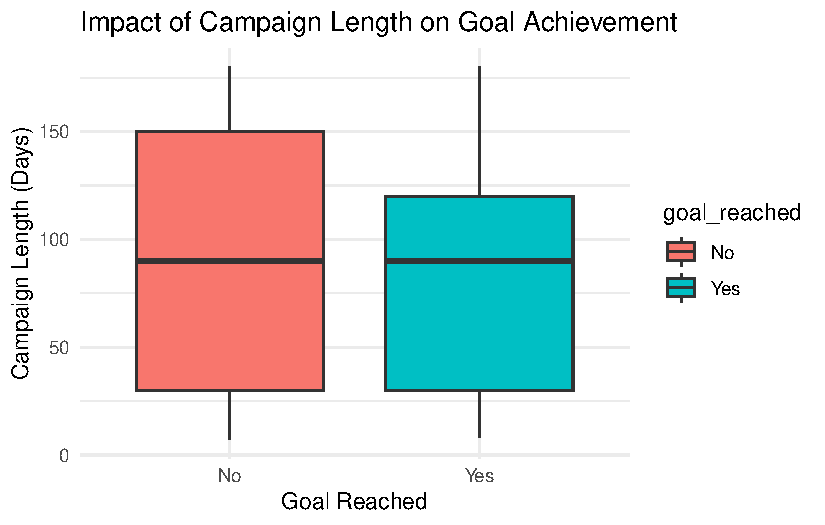
\includegraphics{gfm_data_analysis_files/figure-pdf/time-analysis-1.pdf}

}

\end{figure}

\begin{itemize}
\tightlist
\item
  Both Yes and No Goal reached have very similar
\end{itemize}

\begin{Shaded}
\begin{Highlighting}[]
\NormalTok{time\_analysis}\SpecialCharTok{$}\NormalTok{goal\_reached }\OtherTok{\textless{}{-}} \FunctionTok{factor}\NormalTok{(time\_analysis}\SpecialCharTok{$}\NormalTok{goal\_reached, }\AttributeTok{levels =} \FunctionTok{c}\NormalTok{(}\StringTok{"No"}\NormalTok{, }\StringTok{"Yes"}\NormalTok{))}

\CommentTok{\# Aggregate counts for each unique combination of "campaign\_length\_days" and "goal\_reached"}
\NormalTok{aggregated\_data }\OtherTok{\textless{}{-}} \FunctionTok{aggregate}\NormalTok{(goal\_reached }\SpecialCharTok{\textasciitilde{}}\NormalTok{ campaign\_length\_days, }\AttributeTok{data =}\NormalTok{ time\_analysis, }\AttributeTok{FUN =}\NormalTok{ table)}

\CommentTok{\# Rename the columns}
\FunctionTok{colnames}\NormalTok{(aggregated\_data) }\OtherTok{\textless{}{-}} \FunctionTok{c}\NormalTok{(}\StringTok{"Campaign\_Length\_Days"}\NormalTok{, }\StringTok{"Counts"}\NormalTok{)}

\CommentTok{\# Split "Counts" column into separate columns for "No" and "Yes"}
\NormalTok{aggregated\_data }\OtherTok{\textless{}{-}} \FunctionTok{cbind}\NormalTok{(aggregated\_data, }\FunctionTok{as.data.frame}\NormalTok{(aggregated\_data}\SpecialCharTok{$}\NormalTok{Counts))}

\CommentTok{\# Remove the original "Counts" column}
\NormalTok{aggregated\_data }\OtherTok{\textless{}{-}} \FunctionTok{subset}\NormalTok{(aggregated\_data, }\AttributeTok{select =} \SpecialCharTok{{-}}\NormalTok{Counts)}

\CommentTok{\# Rename the columns for "No" and "Yes"}
\FunctionTok{colnames}\NormalTok{(aggregated\_data)[}\DecValTok{2}\SpecialCharTok{:}\DecValTok{3}\NormalTok{] }\OtherTok{\textless{}{-}} \FunctionTok{c}\NormalTok{(}\StringTok{"No\_Count"}\NormalTok{, }\StringTok{"Yes\_Count"}\NormalTok{)}

\NormalTok{aggregated\_data}\SpecialCharTok{$}\NormalTok{yes\_probability }\OtherTok{\textless{}{-}}\NormalTok{ aggregated\_data}\SpecialCharTok{$}\NormalTok{Yes\_Count }\SpecialCharTok{/}\NormalTok{ (aggregated\_data}\SpecialCharTok{$}\NormalTok{No\_Count }\SpecialCharTok{+}\NormalTok{ aggregated\_data}\SpecialCharTok{$}\NormalTok{Yes\_Count)}

\CommentTok{\# Print the new dataframe}
\FunctionTok{print}\NormalTok{(aggregated\_data)}
\end{Highlighting}
\end{Shaded}

\begin{verbatim}
   Campaign_Length_Days No_Count Yes_Count yes_probability
1                     7        2         0       0.0000000
2                     8        3         2       0.4000000
3                     9        5         0       0.0000000
4                    10        3         1       0.2500000
5                    11        1         1       0.5000000
6                    12        4         2       0.3333333
7                    13        4         1       0.2000000
8                    14        2         2       0.5000000
9                    15        1         4       0.8000000
10                   16        4         2       0.3333333
11                   17        1         3       0.7500000
12                   18        2         3       0.6000000
13                   19        1         1       0.5000000
14                   20        1         1       0.5000000
15                   21        2         2       0.5000000
16                   22        5         3       0.3750000
17                   23        5         3       0.3750000
18                   24        2         2       0.5000000
19                   25        2         2       0.5000000
20                   26        2         3       0.6000000
21                   27        3         3       0.5000000
22                   28        3         1       0.2500000
23                   29        6         0       0.0000000
24                   30      139        76       0.3534884
25                   60      138        84       0.3783784
26                   90      101        95       0.4846939
27                  120      139        64       0.3152709
28                  150      146        78       0.3482143
29                  180       49        16       0.2461538
\end{verbatim}

\begin{Shaded}
\begin{Highlighting}[]
\CommentTok{\# Assuming "aggregated\_data" is your dataframe}

\CommentTok{\# Define the ranges for each group of campaign lengths}
\NormalTok{breaks }\OtherTok{\textless{}{-}} \FunctionTok{c}\NormalTok{(}\DecValTok{0}\NormalTok{, }\DecValTok{7}\NormalTok{, }\DecValTok{14}\NormalTok{, }\DecValTok{21}\NormalTok{, }\DecValTok{30}\NormalTok{, }\DecValTok{60}\NormalTok{, }\DecValTok{90}\NormalTok{, }\DecValTok{120}\NormalTok{, }\DecValTok{150}\NormalTok{, }\DecValTok{180}\NormalTok{)}

\CommentTok{\# Create a new column for the groups}
\NormalTok{aggregated\_data}\SpecialCharTok{$}\NormalTok{weeks }\OtherTok{\textless{}{-}} \FunctionTok{cut}\NormalTok{(aggregated\_data}\SpecialCharTok{$}\NormalTok{Campaign\_Length\_Days, }\AttributeTok{breaks =}\NormalTok{ breaks, }\AttributeTok{labels =} \ConstantTok{FALSE}\NormalTok{)}

\CommentTok{\# Aggregate data based on the groups}
\NormalTok{aggregated\_month\_data }\OtherTok{\textless{}{-}} \FunctionTok{aggregate}\NormalTok{(}\FunctionTok{cbind}\NormalTok{(No\_Count, Yes\_Count) }\SpecialCharTok{\textasciitilde{}}\NormalTok{ weeks, }\AttributeTok{data =}\NormalTok{ aggregated\_data, }\AttributeTok{FUN =}\NormalTok{ sum)}

\NormalTok{aggregated\_month\_data[}\DecValTok{5}\NormalTok{, }\DecValTok{1}\NormalTok{] }\OtherTok{\textless{}{-}} \DecValTok{8}
\NormalTok{aggregated\_month\_data[}\DecValTok{6}\NormalTok{, }\DecValTok{1}\NormalTok{] }\OtherTok{\textless{}{-}} \DecValTok{12}
\NormalTok{aggregated\_month\_data[}\DecValTok{7}\NormalTok{, }\DecValTok{1}\NormalTok{] }\OtherTok{\textless{}{-}} \DecValTok{16}
\NormalTok{aggregated\_month\_data[}\DecValTok{8}\NormalTok{, }\DecValTok{1}\NormalTok{] }\OtherTok{\textless{}{-}} \DecValTok{20}
\NormalTok{aggregated\_month\_data[}\DecValTok{9}\NormalTok{, }\DecValTok{1}\NormalTok{] }\OtherTok{\textless{}{-}} \DecValTok{24}
\FunctionTok{print}\NormalTok{(aggregated\_month\_data)}
\end{Highlighting}
\end{Shaded}

\begin{verbatim}
  weeks No_Count Yes_Count
1     1        2         0
2     2       22         9
3     3       12        16
4     4      167        93
5     8      138        84
6    12      101        95
7    16      139        64
8    20      146        78
9    24       49        16
\end{verbatim}

\begin{Shaded}
\begin{Highlighting}[]
\NormalTok{aggregated\_month\_data}\SpecialCharTok{$}\NormalTok{yes\_probability }\OtherTok{\textless{}{-}}\NormalTok{ aggregated\_month\_data}\SpecialCharTok{$}\NormalTok{Yes\_Count }\SpecialCharTok{/}\NormalTok{ (aggregated\_month\_data}\SpecialCharTok{$}\NormalTok{No\_Count }\SpecialCharTok{+}\NormalTok{ aggregated\_month\_data}\SpecialCharTok{$}\NormalTok{Yes\_Count)}



\CommentTok{\# Create a line plot}
\FunctionTok{ggplot}\NormalTok{(aggregated\_month\_data, }\FunctionTok{aes}\NormalTok{(}\AttributeTok{x =}\NormalTok{ weeks, }\AttributeTok{y =}\NormalTok{ yes\_probability)) }\SpecialCharTok{+}
  \FunctionTok{geom\_line}\NormalTok{() }\SpecialCharTok{+}
  \FunctionTok{scale\_x\_continuous}\NormalTok{(}\AttributeTok{breaks =} \FunctionTok{seq}\NormalTok{(}\FunctionTok{min}\NormalTok{(aggregated\_month\_data}\SpecialCharTok{$}\NormalTok{weeks), }\FunctionTok{max}\NormalTok{(aggregated\_month\_data}\SpecialCharTok{$}\NormalTok{weeks), }\AttributeTok{by =} \DecValTok{1}\NormalTok{)) }\SpecialCharTok{+}
  \FunctionTok{scale\_y\_continuous}\NormalTok{(}\AttributeTok{breaks =} \FunctionTok{seq}\NormalTok{(}\DecValTok{0}\NormalTok{, }\DecValTok{1}\NormalTok{, }\AttributeTok{by =} \FloatTok{0.1}\NormalTok{), }\AttributeTok{limits =} \FunctionTok{c}\NormalTok{(}\DecValTok{0}\NormalTok{, }\DecValTok{1}\NormalTok{)) }\SpecialCharTok{+}
  \FunctionTok{labs}\NormalTok{(}\AttributeTok{x =} \StringTok{"Weeks"}\NormalTok{, }\AttributeTok{y =} \StringTok{"Goal Reached Probability"}\NormalTok{,}
       \AttributeTok{title =} \StringTok{"Goal Reached Probability over Weeks"}\NormalTok{)}
\end{Highlighting}
\end{Shaded}

\begin{figure}[H]

{\centering 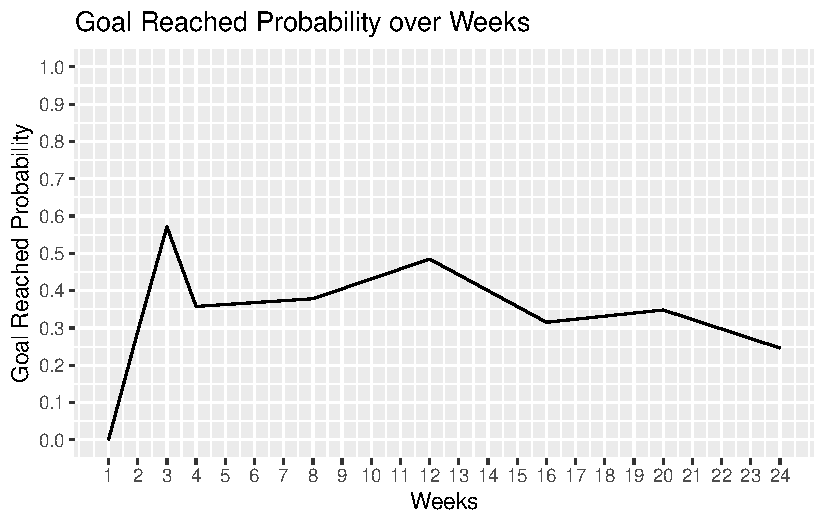
\includegraphics{gfm_data_analysis_files/figure-pdf/time-analysis-2-1.pdf}

}

\end{figure}

\hypertarget{social-media-analysis}{%
\subsection{Social Media Analysis:}\label{social-media-analysis}}

\begin{itemize}
\tightlist
\item
  What is the correlation between social media engagement metrics
  (likes, shares, comments) and the amount of funds raised in GoFundMe
  campaigns?''
\end{itemize}

\begin{Shaded}
\begin{Highlighting}[]
\CommentTok{\#creating dataset }
\NormalTok{sm\_analysis\_data }\OtherTok{\textless{}{-}} \FunctionTok{select}\NormalTok{(gfm\_data, amount\_raised, goal, goal\_reached, FB\_shares, GFM\_hearts)}
\end{Highlighting}
\end{Shaded}

\begin{itemize}
\tightlist
\item
  Does the number of FB\_shares or GFM\_hearts impact the amount that is
  raised?
\end{itemize}

\begin{Shaded}
\begin{Highlighting}[]
\CommentTok{\#scatter plot for FB\_shares vs. amount\_raised }
\FunctionTok{ggplot}\NormalTok{(sm\_analysis\_data, }\FunctionTok{aes}\NormalTok{(}\AttributeTok{x =}\NormalTok{ FB\_shares, }\AttributeTok{y =}\NormalTok{ amount\_raised)) }\SpecialCharTok{+}
  \FunctionTok{geom\_point}\NormalTok{() }\SpecialCharTok{+}
  \FunctionTok{scale\_y\_continuous}\NormalTok{(}\AttributeTok{labels =}\NormalTok{ scales}\SpecialCharTok{::}\FunctionTok{dollar\_format}\NormalTok{()) }\SpecialCharTok{+}
  \FunctionTok{scale\_x\_continuous}\NormalTok{(}\AttributeTok{labels =}\NormalTok{ scales}\SpecialCharTok{::}\NormalTok{comma) }\SpecialCharTok{+}
  \FunctionTok{labs}\NormalTok{(}\AttributeTok{x =} \StringTok{"Facebook Share Amount"}\NormalTok{, }\AttributeTok{y =} \StringTok{"Amount Raised"}\NormalTok{, }\AttributeTok{title =} \StringTok{"FB Shares vs Amount Raised"}\NormalTok{)}
\end{Highlighting}
\end{Shaded}

\begin{verbatim}
Warning: Removed 46 rows containing missing values or values outside the scale range
(`geom_point()`).
\end{verbatim}

\begin{figure}[H]

{\centering 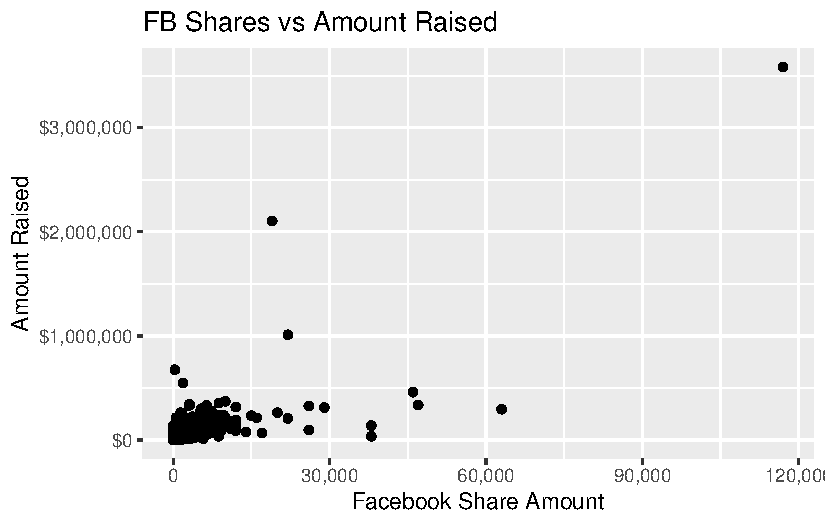
\includegraphics{gfm_data_analysis_files/figure-pdf/social-media-analysis-2-1.pdf}

}

\end{figure}

\begin{itemize}
\tightlist
\item
  The previous graph is hard to interpret, therefore use of log
  transformation is appropriate:
\end{itemize}

\begin{Shaded}
\begin{Highlighting}[]
\CommentTok{\# Create the scatter plot with logarithmic transformations}
\FunctionTok{ggplot}\NormalTok{(sm\_analysis\_data, }\FunctionTok{aes}\NormalTok{(}\AttributeTok{x =} \FunctionTok{log}\NormalTok{(FB\_shares }\SpecialCharTok{+} \DecValTok{1}\NormalTok{), }\AttributeTok{y =} \FunctionTok{log}\NormalTok{(amount\_raised }\SpecialCharTok{+} \DecValTok{1}\NormalTok{))) }\SpecialCharTok{+}
  \FunctionTok{geom\_point}\NormalTok{() }\SpecialCharTok{+}
  \FunctionTok{geom\_smooth}\NormalTok{(}\AttributeTok{method =} \StringTok{"lm"}\NormalTok{, }\AttributeTok{se =} \ConstantTok{FALSE}\NormalTok{, }\FunctionTok{aes}\NormalTok{(}\AttributeTok{group =} \DecValTok{1}\NormalTok{)) }\SpecialCharTok{+}
  \FunctionTok{labs}\NormalTok{(}\AttributeTok{x =} \StringTok{"Log(FB Shares)"}\NormalTok{, }\AttributeTok{y =} \StringTok{"Log(Amount Raised)"}\NormalTok{, }\AttributeTok{title =} \StringTok{"FB Shares vs. Amount Raised with a Log Transformation Applied"}\NormalTok{)}
\end{Highlighting}
\end{Shaded}

\begin{verbatim}
`geom_smooth()` using formula = 'y ~ x'
\end{verbatim}

\begin{verbatim}
Warning: Removed 46 rows containing non-finite outside the scale range
(`stat_smooth()`).
\end{verbatim}

\begin{verbatim}
Warning: Removed 46 rows containing missing values or values outside the scale range
(`geom_point()`).
\end{verbatim}

\begin{figure}[H]

{\centering 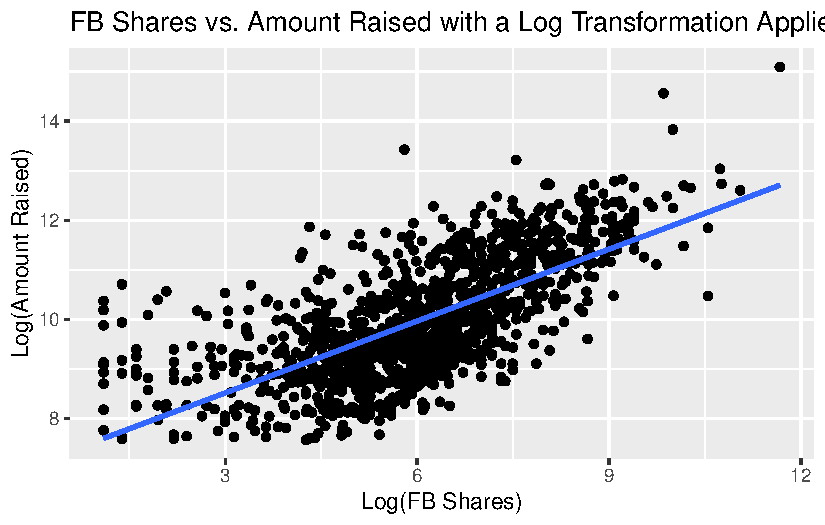
\includegraphics{gfm_data_analysis_files/figure-pdf/social-media-analysis-3-1.pdf}

}

\end{figure}

\begin{itemize}
\tightlist
\item
  The graph above shows that there is a positive correlation between FB
  shares and the amount that is raised.
\end{itemize}

\begin{Shaded}
\begin{Highlighting}[]
\CommentTok{\#sm analysis with outliers removed }
\NormalTok{sm\_no\_outliers }\OtherTok{\textless{}{-}} \FunctionTok{subset}\NormalTok{(sm\_analysis\_data, GFM\_hearts }\SpecialCharTok{\textless{}} \DecValTok{20000}\NormalTok{) }
\CommentTok{\#scatter plot for GFM\_hearts vs. amount\_raised }
\FunctionTok{ggplot}\NormalTok{(sm\_no\_outliers, }\FunctionTok{aes}\NormalTok{(}\AttributeTok{x =}\NormalTok{ GFM\_hearts, }\AttributeTok{y =}\NormalTok{ amount\_raised)) }\SpecialCharTok{+}
  \FunctionTok{geom\_point}\NormalTok{() }\SpecialCharTok{+}
  \FunctionTok{geom\_smooth}\NormalTok{(}\AttributeTok{method =} \StringTok{"lm"}\NormalTok{, }\AttributeTok{se =} \ConstantTok{FALSE}\NormalTok{) }\SpecialCharTok{+}
  \FunctionTok{scale\_y\_continuous}\NormalTok{(}\AttributeTok{labels =}\NormalTok{ scales}\SpecialCharTok{::}\FunctionTok{dollar\_format}\NormalTok{()) }\SpecialCharTok{+}
  \FunctionTok{scale\_x\_continuous}\NormalTok{(}\AttributeTok{labels =}\NormalTok{ scales}\SpecialCharTok{::}\NormalTok{comma) }\SpecialCharTok{+}
  \FunctionTok{labs}\NormalTok{(}\AttributeTok{x =} \StringTok{"Go Fund Me Hearts Amount"}\NormalTok{, }\AttributeTok{y =} \StringTok{"Amount Raised"}\NormalTok{, }\AttributeTok{title =} \StringTok{"GFM Hearts Amount vs Amount Raised"}\NormalTok{, }\AttributeTok{caption =} \StringTok{"Outliers Removed"}\NormalTok{)}
\end{Highlighting}
\end{Shaded}

\begin{verbatim}
`geom_smooth()` using formula = 'y ~ x'
\end{verbatim}

\begin{verbatim}
Warning: Removed 3 rows containing non-finite outside the scale range
(`stat_smooth()`).
\end{verbatim}

\begin{verbatim}
Warning: Removed 3 rows containing missing values or values outside the scale range
(`geom_point()`).
\end{verbatim}

\begin{figure}[H]

{\centering 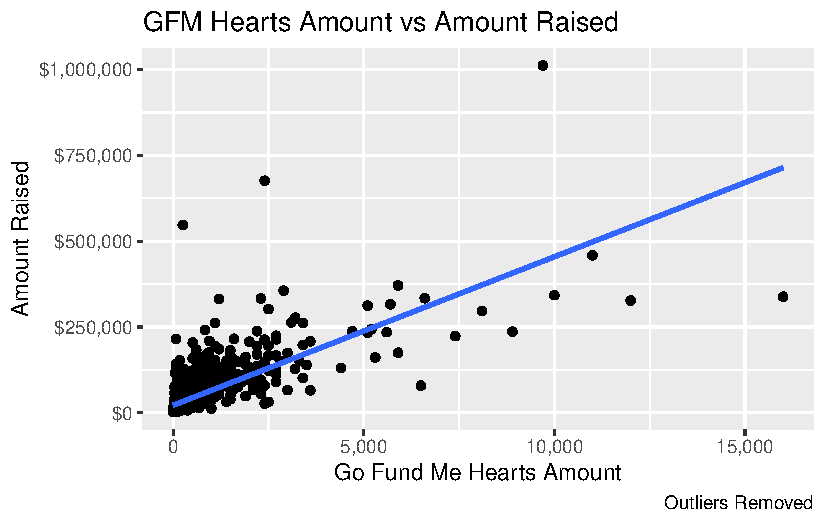
\includegraphics{gfm_data_analysis_files/figure-pdf/social-media-analysis-4-1.pdf}

}

\end{figure}

\begin{itemize}
\tightlist
\item
  The graph shows that there is a positive correlation between the
  number of Go Fund Me hearts and the Amount that the campaign raises.
\end{itemize}

\hypertarget{geographical-analysis}{%
\subsection{Geographical Analysis:}\label{geographical-analysis}}

\begin{itemize}
\tightlist
\item
  Are there discernible geographic patterns in campaign success on
  GoFundMe? Do campaigns in specific regions or cities tend to achieve
  higher fundraising goals?
\end{itemize}

\begin{Shaded}
\begin{Highlighting}[]
\NormalTok{geo\_analysis\_data }\OtherTok{\textless{}{-}} \FunctionTok{select}\NormalTok{(gfm\_data, location, latitude, longitude, amount\_raised, goal, goal\_reached, FB\_shares, GFM\_hearts)}

\NormalTok{geo\_analysis\_data }\OtherTok{\textless{}{-}}\NormalTok{ geo\_analysis\_data[}\SpecialCharTok{!}\FunctionTok{is.na}\NormalTok{(geo\_analysis\_data}\SpecialCharTok{$}\NormalTok{goal\_reached) }\SpecialCharTok{\&}\NormalTok{ geo\_analysis\_data}\SpecialCharTok{$}\NormalTok{goal\_reached }\SpecialCharTok{!=} \StringTok{""}\NormalTok{, ]}

\NormalTok{geo\_analysis\_data }\OtherTok{\textless{}{-}}\NormalTok{ geo\_analysis\_data }\SpecialCharTok{|\textgreater{}}
  \FunctionTok{filter}\NormalTok{(longitude }\SpecialCharTok{\textgreater{}=} \SpecialCharTok{{-}}\DecValTok{140} \SpecialCharTok{\&}\NormalTok{ latitude }\SpecialCharTok{\textgreater{}=} \DecValTok{20}\NormalTok{)}
\end{Highlighting}
\end{Shaded}

\begin{Shaded}
\begin{Highlighting}[]
\NormalTok{usa }\OtherTok{\textless{}{-}} \FunctionTok{map\_data}\NormalTok{(}\StringTok{"usa"}\NormalTok{)}

\FunctionTok{ggplot}\NormalTok{() }\SpecialCharTok{+}
  \FunctionTok{geom\_polygon}\NormalTok{(}\AttributeTok{data =}\NormalTok{ usa, }\FunctionTok{aes}\NormalTok{(}\AttributeTok{x =}\NormalTok{ long, }\AttributeTok{y =}\NormalTok{ lat, }\AttributeTok{group =}\NormalTok{ group), }\AttributeTok{fill =} \StringTok{"lightgrey"}\NormalTok{) }\SpecialCharTok{+}
  \FunctionTok{geom\_point}\NormalTok{(}\AttributeTok{data =}\NormalTok{ geo\_analysis\_data, }\FunctionTok{aes}\NormalTok{(}\AttributeTok{x =}\NormalTok{ longitude, }\AttributeTok{y =}\NormalTok{ latitude, }\AttributeTok{size =}\NormalTok{ amount\_raised, }\AttributeTok{color =}\NormalTok{ goal\_reached), }\AttributeTok{alpha =} \FloatTok{0.5}\NormalTok{) }\SpecialCharTok{+}
  \FunctionTok{scale\_color\_manual}\NormalTok{(}\AttributeTok{values =} \FunctionTok{c}\NormalTok{(}\StringTok{"Yes"} \OtherTok{=} \StringTok{"green"}\NormalTok{, }\StringTok{"No"} \OtherTok{=} \StringTok{"red"}\NormalTok{), }\AttributeTok{name =} \StringTok{"Goal Reached"}\NormalTok{) }\SpecialCharTok{+}
  \FunctionTok{scale\_size}\NormalTok{(}\AttributeTok{name =} \StringTok{"Amount Raised"}\NormalTok{, }\AttributeTok{labels =} \FunctionTok{label\_dollar}\NormalTok{()) }\SpecialCharTok{+}
  \FunctionTok{theme\_minimal}\NormalTok{() }\SpecialCharTok{+}
  \FunctionTok{coord\_fixed}\NormalTok{(}\FloatTok{1.3}\NormalTok{) }\SpecialCharTok{+}  \CommentTok{\# Adjusts the aspect ratio to keep the map looking like the USA}
  \FunctionTok{labs}\NormalTok{(}\AttributeTok{title =} \StringTok{"USA Map with Points Colored and Sized by Goal Reached"}\NormalTok{)}
\end{Highlighting}
\end{Shaded}

\begin{figure}[H]

{\centering 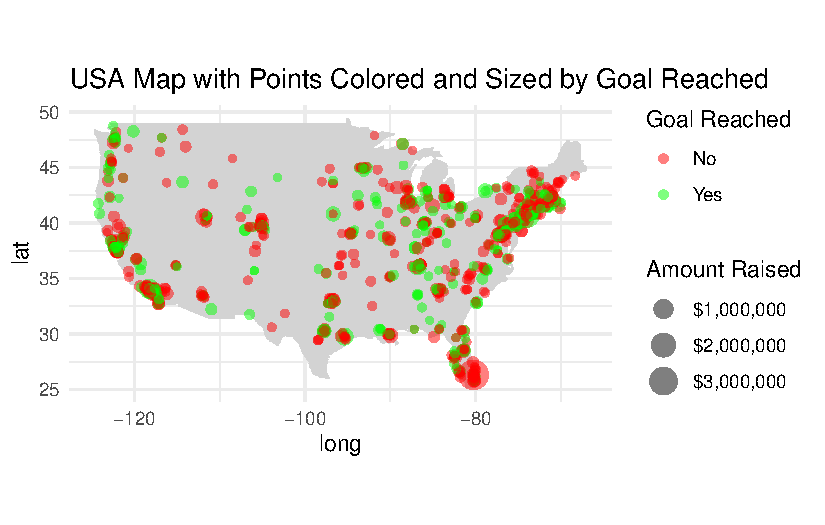
\includegraphics{gfm_data_analysis_files/figure-pdf/geographical-analysis-1-1.pdf}

}

\end{figure}

\hypertarget{text-analysis}{%
\subsection{Text Analysis:}\label{text-analysis}}

\begin{itemize}
\tightlist
\item
  Can the language used in the title and text of the campaign (such as
  sentiment, keywords, urgency) be linked to its success? Are there
  common themes or words in the most successful campaigns?
\end{itemize}

\begin{Shaded}
\begin{Highlighting}[]
\NormalTok{TextDoc }\OtherTok{\textless{}{-}} \FunctionTok{VCorpus}\NormalTok{(}\FunctionTok{VectorSource}\NormalTok{(gfm\_data}\SpecialCharTok{$}\NormalTok{text))}

\CommentTok{\# Convert the text to lower case}
\NormalTok{TextDoc }\OtherTok{\textless{}{-}} \FunctionTok{tm\_map}\NormalTok{(TextDoc, }\FunctionTok{content\_transformer}\NormalTok{(tolower))}
\CommentTok{\# Remove numbers}
\NormalTok{TextDoc }\OtherTok{\textless{}{-}} \FunctionTok{tm\_map}\NormalTok{(TextDoc, removeNumbers)}
\CommentTok{\# Remove english common stopwords}
\NormalTok{TextDoc }\OtherTok{\textless{}{-}} \FunctionTok{tm\_map}\NormalTok{(TextDoc, removeWords, }\FunctionTok{stopwords}\NormalTok{(}\StringTok{"english"}\NormalTok{))}
\NormalTok{TextDoc }\OtherTok{\textless{}{-}} \FunctionTok{tm\_map}\NormalTok{(TextDoc, removeWords, }\FunctionTok{c}\NormalTok{(}\StringTok{"go fund me"}\NormalTok{)) }
\CommentTok{\# Remove punctuations}
\NormalTok{TextDoc }\OtherTok{\textless{}{-}} \FunctionTok{tm\_map}\NormalTok{(TextDoc, removePunctuation)}
\CommentTok{\# Eliminate extra white spaces}
\NormalTok{TextDoc }\OtherTok{\textless{}{-}} \FunctionTok{tm\_map}\NormalTok{(TextDoc, stripWhitespace)}
\CommentTok{\# Text stemming {-} which reduces words to their root form}
\NormalTok{TextDoc }\OtherTok{\textless{}{-}} \FunctionTok{tm\_map}\NormalTok{(TextDoc, stemDocument)}

\CommentTok{\# Build a term{-}document matrix}
\NormalTok{TextDoc\_dtm }\OtherTok{\textless{}{-}} \FunctionTok{TermDocumentMatrix}\NormalTok{(TextDoc)}
\NormalTok{dtm\_m }\OtherTok{\textless{}{-}} \FunctionTok{as.matrix}\NormalTok{(TextDoc\_dtm)}
\CommentTok{\# Sort by descearing value of frequency}
\NormalTok{dtm\_v }\OtherTok{\textless{}{-}} \FunctionTok{sort}\NormalTok{(}\FunctionTok{rowSums}\NormalTok{(dtm\_m),}\AttributeTok{decreasing=}\ConstantTok{TRUE}\NormalTok{)}
\NormalTok{dtm\_d }\OtherTok{\textless{}{-}} \FunctionTok{data.frame}\NormalTok{(}\AttributeTok{word =} \FunctionTok{names}\NormalTok{(dtm\_v),}\AttributeTok{freq=}\NormalTok{dtm\_v)}
\CommentTok{\# Display the top 5 most frequent words}
\FunctionTok{head}\NormalTok{(dtm\_d, }\DecValTok{10}\NormalTok{)}
\end{Highlighting}
\end{Shaded}

\begin{verbatim}
           word freq
help       help 1675
need       need 1415
today     today 1270
famili   famili  456
fund       fund  359
year       year  356
will       will  310
friend   friend  261
love       love  233
support support  233
\end{verbatim}

\begin{Shaded}
\begin{Highlighting}[]
\FunctionTok{barplot}\NormalTok{(dtm\_d[}\DecValTok{1}\SpecialCharTok{:}\DecValTok{10}\NormalTok{,]}\SpecialCharTok{$}\NormalTok{freq, }\AttributeTok{las =} \DecValTok{2}\NormalTok{, }\AttributeTok{names.arg =}\NormalTok{ dtm\_d[}\DecValTok{1}\SpecialCharTok{:}\DecValTok{10}\NormalTok{,]}\SpecialCharTok{$}\NormalTok{word,}
        \AttributeTok{col =}\StringTok{"lightgreen"}\NormalTok{, }\AttributeTok{main =}\StringTok{"Top 10 most frequent words"}\NormalTok{,}
        \AttributeTok{ylab =} \StringTok{"Word frequencies"}\NormalTok{)}
\end{Highlighting}
\end{Shaded}

\begin{figure}[H]

{\centering 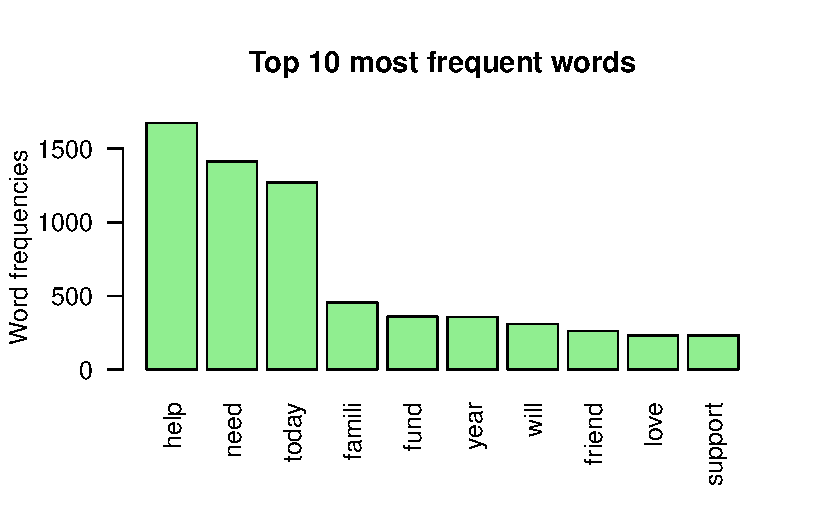
\includegraphics{gfm_data_analysis_files/figure-pdf/unnamed-chunk-11-1.pdf}

}

\end{figure}

\hfill\break

\begin{Shaded}
\begin{Highlighting}[]
\FunctionTok{set.seed}\NormalTok{(}\DecValTok{1234}\NormalTok{)}
\FunctionTok{wordcloud}\NormalTok{(}\AttributeTok{words =}\NormalTok{ dtm\_d}\SpecialCharTok{$}\NormalTok{word, }\AttributeTok{freq =}\NormalTok{ dtm\_d}\SpecialCharTok{$}\NormalTok{freq, }\AttributeTok{min.freq =} \DecValTok{5}\NormalTok{,}
          \AttributeTok{max.words=}\DecValTok{100}\NormalTok{, }\AttributeTok{random.order=}\ConstantTok{FALSE}\NormalTok{, }\AttributeTok{rot.per=}\FloatTok{0.40}\NormalTok{, }
          \AttributeTok{colors=}\FunctionTok{brewer.pal}\NormalTok{(}\DecValTok{8}\NormalTok{, }\StringTok{"Dark2"}\NormalTok{))}
\end{Highlighting}
\end{Shaded}

\begin{figure}[H]

{\centering 
\includegraphics{gfm_data_analysis_files/figure-pdf/unnamed-chunk-12-1.pdf}

}

\end{figure}

\begin{itemize}
\tightlist
\item
  Can sentiment analysis of campaign descriptions provide insights into
  campaign success on GoFundMe? How do positive or negative sentiments
  affect donor engagement and fundraising outcomes?''
\end{itemize}

\hypertarget{fundraising-goals-and-donor-engagement-analysis}{%
\subsection{Fundraising Goals and Donor Engagement
Analysis:}\label{fundraising-goals-and-donor-engagement-analysis}}

\begin{itemize}
\item
  How do different initial fundraising goals impact the number of
  donations received and donor engagement on GoFundMe?
\item
  Are there certain categories of campaigns that perform better than
  others?
\end{itemize}

\begin{Shaded}
\begin{Highlighting}[]
\NormalTok{gfm\_cleaned\_data }\OtherTok{\textless{}{-}} \FunctionTok{read.csv}\NormalTok{(}\StringTok{"data/gfm\_cleaned\_data.csv"}\NormalTok{)}
\end{Highlighting}
\end{Shaded}

\hypertarget{how-do-different-initial-fundraising-goals-impact-the-number-of-donations-received-and-donor-engagement-on-gofundme}{%
\subsection{How do different initial fundraising goals impact the number
of donations received and donor engagement on
GoFundMe?}\label{how-do-different-initial-fundraising-goals-impact-the-number-of-donations-received-and-donor-engagement-on-gofundme}}

\begin{Shaded}
\begin{Highlighting}[]
\CommentTok{\# Check for missing values in the goal and number\_of\_donators variables}
\FunctionTok{sum}\NormalTok{(}\FunctionTok{is.na}\NormalTok{(gfm\_cleaned\_data}\SpecialCharTok{$}\NormalTok{goal))}
\end{Highlighting}
\end{Shaded}

\begin{verbatim}
[1] 7
\end{verbatim}

\begin{Shaded}
\begin{Highlighting}[]
\FunctionTok{sum}\NormalTok{(}\FunctionTok{is.na}\NormalTok{(gfm\_cleaned\_data}\SpecialCharTok{$}\NormalTok{number\_of\_donators))}
\end{Highlighting}
\end{Shaded}

\begin{verbatim}
[1] 7
\end{verbatim}

\begin{Shaded}
\begin{Highlighting}[]
\CommentTok{\# Remove rows with missing values in \textquotesingle{}goal\textquotesingle{} and \textquotesingle{}number\_of\_donators\textquotesingle{}}
\NormalTok{gfm\_cleaned\_data\_1 }\OtherTok{\textless{}{-}} \FunctionTok{na.omit}\NormalTok{(gfm\_cleaned\_data[, }\FunctionTok{c}\NormalTok{(}\StringTok{"goal"}\NormalTok{, }\StringTok{"number\_of\_donators"}\NormalTok{)])}

\CommentTok{\# Check if missing values are removed}
\FunctionTok{sum}\NormalTok{(}\FunctionTok{is.na}\NormalTok{(gfm\_cleaned\_data\_1}\SpecialCharTok{$}\NormalTok{goal))}
\end{Highlighting}
\end{Shaded}

\begin{verbatim}
[1] 0
\end{verbatim}

\begin{Shaded}
\begin{Highlighting}[]
\FunctionTok{sum}\NormalTok{(}\FunctionTok{is.na}\NormalTok{(gfm\_cleaned\_data\_1}\SpecialCharTok{$}\NormalTok{number\_of\_donators))}
\end{Highlighting}
\end{Shaded}

\begin{verbatim}
[1] 0
\end{verbatim}

\begin{Shaded}
\begin{Highlighting}[]
\CommentTok{\# Correlation analysis between initial fundraising goals and number of donations}
\NormalTok{correlation\_donations }\OtherTok{\textless{}{-}} \FunctionTok{cor}\NormalTok{(gfm\_cleaned\_data\_1}\SpecialCharTok{$}\NormalTok{goal, gfm\_cleaned\_data\_1}\SpecialCharTok{$}\NormalTok{number\_of\_donators)}
\NormalTok{correlation\_donations}
\end{Highlighting}
\end{Shaded}

\begin{verbatim}
[1] 0.5419016
\end{verbatim}

\emph{Removing rows with missing values can have several implications}:

\emph{Reduced Sample Size:} Removing rows with missing values decreases
the size of your dataset, which can reduce the statistical power of your
analysis. A smaller sample size may lead to less reliable estimates and
wider confidence intervals.

\emph{Bias:} If the missing values are not completely at random (MCAR)
and are related to the variables being analyzed, removing them can
introduce bias into your analysis. This bias can distort the
relationships between variables and lead to erroneous conclusions.

\emph{Loss of Information:} By removing rows with missing values, you
lose information that could potentially be valuable for your analysis.
This loss of information can reduce the completeness of your dataset and
limit the insights that can be gained from it.

\emph{Misrepresentation of Results:} Removing missing values can alter
the distribution and characteristics of your data, potentially leading
to a misrepresentation of the true population characteristics. This
misrepresentation can affect the generalizability of your results.

\emph{Assumption Violation:} Some statistical methods assume that the
data are complete and free of missing values. Removing missing values to
satisfy these assumptions may violate the integrity of your analysis and
lead to invalid results.

\hypertarget{correlation-analysis-results}{%
\subsection{correlation analysis
results}\label{correlation-analysis-results}}

A correlation coefficient of approximately 0.5419 indicates a moderate
positive correlation between the initial fundraising goals and the
number of donations received on GoFundMe. Here's how you can interpret
this correlation coefficient:

\emph{Strength of the Relationship:} The correlation coefficient ranges
from -1 to 1. A value of 0.5419 suggests a moderate positive
relationship between initial fundraising goals and the number of
donations. This indicates that as the initial fundraising goals
increase, the number of donations tends to increase as well, and vice
versa.

\emph{Direction of the Relationship:} The positive sign indicates that
as one variable (initial fundraising goals) increases, the other
variable (number of donations) tends to increase as well. In other
words, campaigns with higher initial fundraising goals tend to attract
more donations.

\begin{Shaded}
\begin{Highlighting}[]
\CommentTok{\# Linear regression analysis}
\NormalTok{linear\_model }\OtherTok{\textless{}{-}} \FunctionTok{lm}\NormalTok{(number\_of\_donators }\SpecialCharTok{\textasciitilde{}}\NormalTok{ goal, }\AttributeTok{data =}\NormalTok{ gfm\_cleaned\_data)}

\CommentTok{\# Summary of the linear model}
\FunctionTok{summary}\NormalTok{(linear\_model)}
\end{Highlighting}
\end{Shaded}

\begin{verbatim}

Call:
lm(formula = number_of_donators ~ goal, data = gfm_cleaned_data)

Residuals:
     Min       1Q   Median       3Q      Max 
-15512.8   -203.9   -142.2     -0.1  30886.7 

Coefficients:
             Estimate Std. Error t value Pr(>|t|)    
(Intercept) 1.742e+02  5.099e+01   3.416 0.000656 ***
goal        4.951e-03  2.190e-04  22.604  < 2e-16 ***
---
Signif. codes:  0 '***' 0.001 '**' 0.01 '*' 0.05 '.' 0.1 ' ' 1

Residual standard error: 1683 on 1229 degrees of freedom
  (7 observations deleted due to missingness)
Multiple R-squared:  0.2937,    Adjusted R-squared:  0.2931 
F-statistic: 510.9 on 1 and 1229 DF,  p-value: < 2.2e-16
\end{verbatim}

The linear regression model results provide insights into the
relationship between the initial fundraising goals and the number of
donators on GoFundMe.

\emph{Intercept:} The intercept represents the expected number of
donators when the initial fundraising goal is zero. In this case, the
intercept is approximately 174.2 (rounded from 1.742e+02). This
intercept value may not have practical meaning since initial fundraising
goals are unlikely to be zero in real-world scenarios.

\emph{Coefficients:} The coefficient for the goal variable represents
the change in the number of donators for a one-unit increase in the
initial fundraising goal. For every one-unit increase in the initial
fundraising goal, the number of donators is expected to increase by
approximately 0.005 (rounded from 4.951e-03). The coefficient is highly
significant (p-value \textless{} 2e-16), indicating a strong association
between the initial fundraising goal and the number of donators.

\emph{Residuals:} Residuals represent the differences between the
observed values and the values predicted by the regression model. The
residuals have a mean close to zero, indicating that the model is
unbiased on average. The range of residuals indicates the spread of
errors around the regression line.

\emph{Model Fit:} The adjusted R-squared value (0.2931) indicates that
approximately 29.31\% of the variation in the number of donators can be
explained by the initial fundraising goals. The F-statistic (510.9) is
significant (p-value \textless{} 2.2e-16), suggesting that the
regression model as a whole is statistically significant in explaining
the relationship between the variables.

\emph{Overall Interpretation:} The linear regression model suggests that
there is a statistically significant positive relationship between the
initial fundraising goals and the number of donators on GoFundMe.
However, it's important to note that the model's explanatory power
(adjusted R-squared) is relatively low, indicating that other factors
not included in the model may also influence the number of donators.

Additionally, while the relationship is statistically significant, the
coefficient for the goal variable is small, suggesting that the
practical significance of the relationship may be limited.

In conclusion, while the model indicates a significant association
between initial fundraising goals and the number of donators, further
investigation into additional factors influencing donation behavior may
provide a more comprehensive understanding of donor engagement on
GoFundMe.

\begin{Shaded}
\begin{Highlighting}[]
\CommentTok{\# Define a custom theme for the plot}
\NormalTok{custom\_theme }\OtherTok{\textless{}{-}} \FunctionTok{theme\_minimal}\NormalTok{() }\SpecialCharTok{+}
  \FunctionTok{theme}\NormalTok{(}
    \AttributeTok{panel.grid.major =} \FunctionTok{element\_blank}\NormalTok{(),}
    \AttributeTok{panel.grid.minor =} \FunctionTok{element\_blank}\NormalTok{(),}
    \AttributeTok{axis.line =} \FunctionTok{element\_line}\NormalTok{(}\AttributeTok{size =} \FloatTok{0.5}\NormalTok{, }\AttributeTok{color =} \StringTok{"black"}\NormalTok{),}
    \AttributeTok{axis.text =} \FunctionTok{element\_text}\NormalTok{(}\AttributeTok{size =} \DecValTok{10}\NormalTok{),}
    \AttributeTok{axis.title =} \FunctionTok{element\_text}\NormalTok{(}\AttributeTok{size =} \DecValTok{12}\NormalTok{),}
    \AttributeTok{plot.title =} \FunctionTok{element\_text}\NormalTok{(}\AttributeTok{size =} \DecValTok{14}\NormalTok{, }\AttributeTok{hjust =} \FloatTok{0.5}\NormalTok{),}
    \AttributeTok{plot.subtitle =} \FunctionTok{element\_text}\NormalTok{(}\AttributeTok{size =} \DecValTok{12}\NormalTok{, }\AttributeTok{hjust =} \FloatTok{0.5}\NormalTok{)}
\NormalTok{  )}
\end{Highlighting}
\end{Shaded}

\begin{verbatim}
Warning: The `size` argument of `element_line()` is deprecated as of ggplot2 3.4.0.
i Please use the `linewidth` argument instead.
\end{verbatim}

\begin{Shaded}
\begin{Highlighting}[]
\CommentTok{\# Plotting initial fundraising goals vs. number of donations with improved aesthetics}
\FunctionTok{ggplot}\NormalTok{(gfm\_cleaned\_data, }\FunctionTok{aes}\NormalTok{(}\AttributeTok{x =}\NormalTok{ goal, }\AttributeTok{y =}\NormalTok{ number\_of\_donators)) }\SpecialCharTok{+}
  \FunctionTok{geom\_point}\NormalTok{(}\AttributeTok{color =} \StringTok{"grey2"}\NormalTok{, }\AttributeTok{alpha =} \FloatTok{0.7}\NormalTok{) }\SpecialCharTok{+} 
  \FunctionTok{geom\_smooth}\NormalTok{(}\AttributeTok{method =} \StringTok{"lm"}\NormalTok{, }\AttributeTok{color =} \StringTok{"salmon"}\NormalTok{) }\SpecialCharTok{+}  
  \FunctionTok{labs}\NormalTok{(}\AttributeTok{x =} \StringTok{"Initial Fundraising Goal ($)"}\NormalTok{, }\AttributeTok{y =} \StringTok{"Number of Donations"}\NormalTok{) }\SpecialCharTok{+}
  \FunctionTok{ggtitle}\NormalTok{(}\StringTok{"Initial Fundraising Goal vs. Number of Donations"}\NormalTok{) }\SpecialCharTok{+}
  \FunctionTok{scale\_x\_continuous}\NormalTok{(}\AttributeTok{labels =}\NormalTok{ dollar) }\SpecialCharTok{+}  
\NormalTok{  custom\_theme  }
\end{Highlighting}
\end{Shaded}

\begin{verbatim}
`geom_smooth()` using formula = 'y ~ x'
\end{verbatim}

\begin{verbatim}
Warning: Removed 7 rows containing non-finite outside the scale range
(`stat_smooth()`).
\end{verbatim}

\begin{verbatim}
Warning: Removed 7 rows containing missing values or values outside the scale range
(`geom_point()`).
\end{verbatim}

\begin{figure}[H]

{\centering 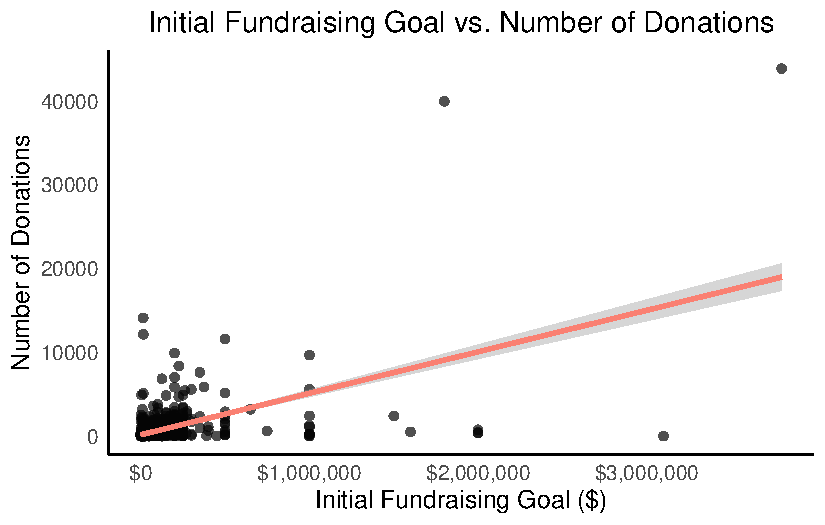
\includegraphics{gfm_data_analysis_files/figure-pdf/unnamed-chunk-18-1.pdf}

}

\end{figure}

\begin{Shaded}
\begin{Highlighting}[]
\CommentTok{\# Remove missing values from \textquotesingle{}goal\textquotesingle{}, \textquotesingle{}GFM\_hearts\textquotesingle{}, and "FB\_shares" variables}
\NormalTok{complete\_data }\OtherTok{\textless{}{-}} \FunctionTok{na.omit}\NormalTok{(gfm\_cleaned\_data[, }\FunctionTok{c}\NormalTok{(}\StringTok{"goal"}\NormalTok{, }\StringTok{"GFM\_hearts"}\NormalTok{, }\StringTok{"FB\_shares"}\NormalTok{)])}

\CommentTok{\# Correlation analysis between initial fundraising goals and donor engagement (GFM hearts)}
\NormalTok{correlation\_engagement\_hearts }\OtherTok{\textless{}{-}} \FunctionTok{cor}\NormalTok{(complete\_data}\SpecialCharTok{$}\NormalTok{goal, complete\_data}\SpecialCharTok{$}\NormalTok{GFM\_hearts, }\AttributeTok{use =} \StringTok{"pairwise.complete.obs"}\NormalTok{)}

\NormalTok{correlation\_engagement\_hearts}
\end{Highlighting}
\end{Shaded}

\begin{verbatim}
[1] 0.5414683
\end{verbatim}

With a correlation coefficient of approximately 0.5415, the
interpretation remains largely the same:

\emph{Strength of the Relationship:} The correlation coefficient of
0.5415 still indicates a moderate positive relationship between the
initial fundraising goals and donor engagement (represented by the
GFM\_hearts variable). This suggests that as the initial fundraising
goals increase, the donor engagement tends to increase as well, and vice
versa.

\emph{Direction of the Relationship:} The positive sign indicates that
as one variable (initial fundraising goals) increases, the other
variable (donor engagement) tends to increase as well. In other words,
campaigns with higher initial fundraising goals tend to attract more
donor engagement in terms of GFM hearts.

\begin{Shaded}
\begin{Highlighting}[]
\CommentTok{\# Correlation analysis between initial fundraising goals and donor engagement (FB\_shares)}
\NormalTok{correlation\_engagement\_shares }\OtherTok{\textless{}{-}} \FunctionTok{cor}\NormalTok{(complete\_data}\SpecialCharTok{$}\NormalTok{goal, complete\_data}\SpecialCharTok{$}\NormalTok{FB\_shares, }\AttributeTok{use =} \StringTok{"pairwise.complete.obs"}\NormalTok{)}

\NormalTok{correlation\_engagement\_shares}
\end{Highlighting}
\end{Shaded}

\begin{verbatim}
[1] 0.4647916
\end{verbatim}

With a correlation coefficient of approximately 0.4648:

\emph{Strength of the Relationship:} The correlation coefficient of
0.4648 indicates a moderate positive relationship between the initial
fundraising goals and donor engagement through Facebook shares. This
suggests that as the initial fundraising goals increase, the number of
Facebook shares tends to increase as well, and vice versa.

\emph{Direction of the Relationship:} The positive sign indicates that
as one variable (initial fundraising goals) increases, the other
variable (Facebook shares) tends to increase as well. In other words,
campaigns with higher initial fundraising goals tend to attract more
donor engagement in terms of Facebook shares.

\begin{Shaded}
\begin{Highlighting}[]
\CommentTok{\# Linear regression analysis for donor engagement (GFM\_hearts)}
\NormalTok{linear\_model\_engagement\_hearts }\OtherTok{\textless{}{-}} \FunctionTok{lm}\NormalTok{(GFM\_hearts }\SpecialCharTok{\textasciitilde{}}\NormalTok{ goal, }\AttributeTok{data =}\NormalTok{ complete\_data)  }

\CommentTok{\# Summary of the linear model for donor engagement}
\FunctionTok{summary}\NormalTok{(linear\_model\_engagement\_hearts)}
\end{Highlighting}
\end{Shaded}

\begin{verbatim}

Call:
lm(formula = GFM_hearts ~ goal, data = complete_data)

Residuals:
     Min       1Q   Median       3Q      Max 
-15779.6   -219.7   -151.9      2.2  30754.7 

Coefficients:
             Estimate Std. Error t value Pr(>|t|)    
(Intercept) 1.853e+02  5.319e+01   3.485 0.000511 ***
goal        5.033e-03  2.265e-04  22.217  < 2e-16 ***
---
Signif. codes:  0 '***' 0.001 '**' 0.01 '*' 0.05 '.' 0.1 ' ' 1

Residual standard error: 1726 on 1190 degrees of freedom
Multiple R-squared:  0.2932,    Adjusted R-squared:  0.2926 
F-statistic: 493.6 on 1 and 1190 DF,  p-value: < 2.2e-16
\end{verbatim}

The linear regression model for donor engagement (represented by
GFM\_hearts) yields the following results:

\emph{Intercept:} The intercept of approximately 185.3 (rounded from
1.853e+02) indicates the estimated number of GFM hearts when the initial
fundraising goal is zero. However, this value may not have practical
meaning, as initial fundraising goals are unlikely to be zero.

\emph{Goal Coefficient:} The coefficient for the goal variable is
approximately 0.005 (rounded from 5.033e-03). This means that for every
one-unit increase in the initial fundraising goal, the number of GFM
hearts is expected to increase by approximately 0.005.

\emph{Significance:} Both the intercept and the coefficient for the goal
variable are highly significant (p-value \textless{} 0.001), indicating
a strong association between the initial fundraising goals and donor
engagement (GFM hearts).

\emph{Model Fit:} The adjusted R-squared value is 0.2926, indicating
that approximately 29.26\% of the variation in donor engagement (GFM
hearts) can be explained by the initial fundraising goals. The
F-statistic is significant (p-value \textless{} 0.001), suggesting that
the regression model as a whole is statistically significant in
explaining the relationship between the variables.

\emph{Residuals:} The residuals have a mean close to zero, indicating
that the model is unbiased on average. The residual standard error is
approximately 1726, indicating the average distance that the observed
values deviate from the predicted values.

In summary, the linear regression model suggests that there is a
statistically significant positive relationship between the initial
fundraising goals and donor engagement (GFM hearts). However, the
explanatory power of the model (adjusted R-squared) is relatively low,
indicating that other factors not included in the model may also
influence donor engagement behavior. Further analysis and interpretation
within the context of your dataset and domain knowledge are recommended
for a comprehensive understanding of the relationship between these
variables.

\begin{Shaded}
\begin{Highlighting}[]
\CommentTok{\# Linear regression analysis for donor engagement (FB\_shares)}
\NormalTok{linear\_model\_engagement\_shares }\OtherTok{\textless{}{-}} \FunctionTok{lm}\NormalTok{(FB\_shares }\SpecialCharTok{\textasciitilde{}}\NormalTok{ goal, }\AttributeTok{data =}\NormalTok{ complete\_data)  }

\CommentTok{\# Summary of the linear model for donor engagement}
\FunctionTok{summary}\NormalTok{(linear\_model\_engagement\_shares)}
\end{Highlighting}
\end{Shaded}

\begin{verbatim}

Call:
lm(formula = FB_shares ~ goal, data = complete_data)

Residuals:
   Min     1Q Median     3Q    Max 
-35137   -893   -709   -121  74109 

Coefficients:
             Estimate Std. Error t value Pr(>|t|)    
(Intercept) 8.102e+02  1.436e+02   5.643 2.08e-08 ***
goal        1.107e-02  6.115e-04  18.108  < 2e-16 ***
---
Signif. codes:  0 '***' 0.001 '**' 0.01 '*' 0.05 '.' 0.1 ' ' 1

Residual standard error: 4658 on 1190 degrees of freedom
Multiple R-squared:  0.216, Adjusted R-squared:  0.2154 
F-statistic: 327.9 on 1 and 1190 DF,  p-value: < 2.2e-16
\end{verbatim}

The linear regression model for donor engagement (represented by
FB\_shares) yields the following results:

\emph{Intercept:} The intercept of approximately 810.2 (rounded from
8.102e+02) indicates the estimated number of Facebook shares when the
initial fundraising goal is zero. However, this value may not have
practical meaning, as initial fundraising goals are unlikely to be zero.

\emph{Goal Coefficient:} The coefficient for the goal variable is
approximately 0.0111 (rounded from 1.107e-02). This means that for every
one-unit increase in the initial fundraising goal, the number of
Facebook shares is expected to increase by approximately 0.0111.

\emph{Significance:} Both the intercept and the coefficient for the goal
variable are highly significant (p-value \textless{} 0.001), indicating
a strong association between the initial fundraising goals and donor
engagement (Facebook shares).

\emph{Model Fit:} The adjusted R-squared value is 0.2154, indicating
that approximately 21.54\% of the variation in donor engagement
(Facebook shares) can be explained by the initial fundraising goals. The
F-statistic is significant (p-value \textless{} 0.001), suggesting that
the regression model as a whole is statistically significant in
explaining the relationship between the variables.

\emph{Residuals:} The residuals have a mean close to zero, indicating
that the model is unbiased on average. The residual standard error is
approximately 4658, indicating the average distance that the observed
values deviate from the predicted values.

In summary, the linear regression model suggests that there is a
statistically significant positive relationship between the initial
fundraising goals and donor engagement (Facebook shares). However,
similar to the previous model, the explanatory power of the model
(adjusted R-squared) is relatively low, indicating that other factors
not included in the model may also influence donor engagement behavior.
Further analysis and interpretation within the context of your dataset
and domain knowledge are recommended for a comprehensive understanding
of the relationship between these variables.

\hypertarget{are-there-certain-categories-of-campaigns-that-perform-better-than-others}{%
\subsection{Are there certain categories of campaigns that perform
better than
others?}\label{are-there-certain-categories-of-campaigns-that-perform-better-than-others}}

\begin{Shaded}
\begin{Highlighting}[]
\CommentTok{\# Group data by category and calculate aggregate statistics}
\NormalTok{category\_performance }\OtherTok{\textless{}{-}}\NormalTok{ gfm\_cleaned\_data }\SpecialCharTok{\%\textgreater{}\%}
  \FunctionTok{group\_by}\NormalTok{(category) }\SpecialCharTok{\%\textgreater{}\%}
  \FunctionTok{summarise}\NormalTok{(}
    \AttributeTok{mean\_goal =} \FunctionTok{mean}\NormalTok{(goal),}
    \AttributeTok{mean\_donators =} \FunctionTok{mean}\NormalTok{(number\_of\_donators),}
    \AttributeTok{mean\_FB\_shares =} \FunctionTok{mean}\NormalTok{(FB\_shares),}
    \AttributeTok{mean\_GFM\_hearts =} \FunctionTok{mean}\NormalTok{(GFM\_hearts)}
\NormalTok{  ) }

\CommentTok{\# Reorder categories based on mean number of donations}
\NormalTok{category\_performance }\OtherTok{\textless{}{-}}\NormalTok{ category\_performance }\SpecialCharTok{\%\textgreater{}\%}
  \FunctionTok{mutate}\NormalTok{(}\AttributeTok{category =} \FunctionTok{factor}\NormalTok{(category, }\AttributeTok{levels =}\NormalTok{ category[}\FunctionTok{order}\NormalTok{(}\SpecialCharTok{{-}}\NormalTok{mean\_donators)]))}

\NormalTok{category\_performance }\OtherTok{\textless{}{-}} \FunctionTok{na.omit}\NormalTok{(category\_performance)}

\NormalTok{category\_performance }
\end{Highlighting}
\end{Shaded}

\begin{verbatim}
# A tibble: 9 x 5
  category  mean_goal mean_donators mean_FB_shares mean_GFM_hearts
  <fct>         <dbl>         <dbl>          <dbl>           <dbl>
1 Animals      98500          1424           5413.           1367.
2 Business     36416.          117.           438.            117.
3 Charity     171995.          664.          1522.            639.
4 Education    62326.          349.           832.            351.
5 Emergency   152998.         1466.          4214.           1481.
6 Family       77056.          721.          2642.            743.
7 Medical     199736.         1618.          4032            1637.
8 Memorial    112639.         1593.          5915.           1664.
9 Volunteer    46422.          145.           706.            150.
\end{verbatim}

\begin{Shaded}
\begin{Highlighting}[]
\CommentTok{\# Bar chart for mean fundraising goals by category}
\FunctionTok{ggplot}\NormalTok{(category\_performance, }\FunctionTok{aes}\NormalTok{(}\AttributeTok{x =}\NormalTok{ category, }\AttributeTok{y =}\NormalTok{ mean\_donators)) }\SpecialCharTok{+}
  \FunctionTok{geom\_bar}\NormalTok{(}\AttributeTok{stat =} \StringTok{"identity"}\NormalTok{, }\AttributeTok{fill =} \StringTok{"skyblue"}\NormalTok{) }\SpecialCharTok{+}
  \FunctionTok{labs}\NormalTok{(}\AttributeTok{x =} \StringTok{"Category"}\NormalTok{, }\AttributeTok{y =} \StringTok{"Mean Number of Donations"}\NormalTok{, }
       \AttributeTok{title =} \StringTok{"Mean Number of Donations by Category"}\NormalTok{) }\SpecialCharTok{+}
  \FunctionTok{theme}\NormalTok{(}\AttributeTok{axis.text.x =} \FunctionTok{element\_text}\NormalTok{(}\AttributeTok{angle =} \DecValTok{45}\NormalTok{, }\AttributeTok{hjust =} \DecValTok{1}\NormalTok{))}
\end{Highlighting}
\end{Shaded}

\begin{figure}[H]

{\centering 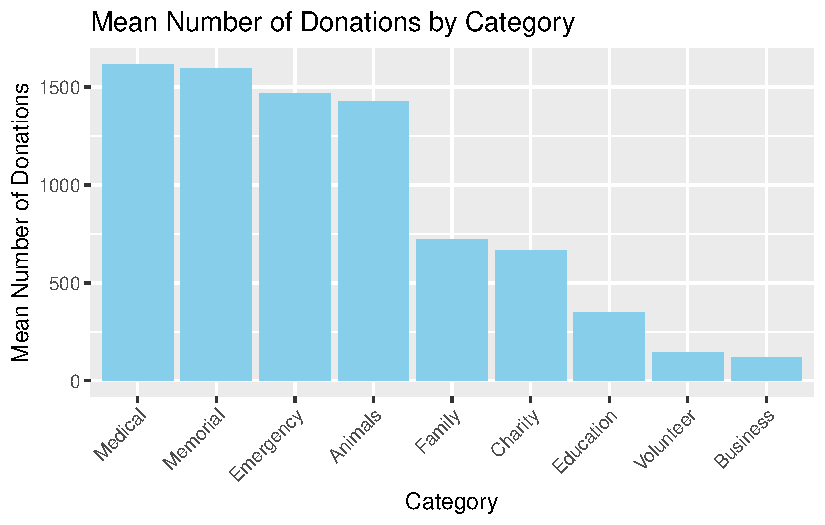
\includegraphics{gfm_data_analysis_files/figure-pdf/unnamed-chunk-24-1.pdf}

}

\end{figure}

\begin{Shaded}
\begin{Highlighting}[]
\CommentTok{\# Remove rows with NA values in \textquotesingle{}number\_of\_donators\textquotesingle{}}
\NormalTok{anova\_clean }\OtherTok{\textless{}{-}} \FunctionTok{na.omit}\NormalTok{(gfm\_cleaned\_data[, }\FunctionTok{c}\NormalTok{(}\StringTok{"number\_of\_donators"}\NormalTok{, }\StringTok{"category"}\NormalTok{)])}

\CommentTok{\# Perform one{-}way ANOVA}
\NormalTok{anova\_model }\OtherTok{\textless{}{-}} \FunctionTok{aov}\NormalTok{(number\_of\_donators }\SpecialCharTok{\textasciitilde{}}\NormalTok{ category, }\AttributeTok{data =}\NormalTok{ anova\_clean)}
\FunctionTok{summary}\NormalTok{(anova\_model)}
\end{Highlighting}
\end{Shaded}

\begin{verbatim}
              Df    Sum Sq  Mean Sq F value Pr(>F)    
category      17 4.665e+08 27440067   7.456 <2e-16 ***
Residuals   1213 4.464e+09  3680324                   
---
Signif. codes:  0 '***' 0.001 '**' 0.01 '*' 0.05 '.' 0.1 ' ' 1
\end{verbatim}

The results of the ANOVA test with removed NA values in the
number\_of\_donators column show that there is a significant difference
in the mean number of donations between the campaign categories (p
\textless{} 0.001). This confirms that the significant difference
observed in the original ANOVA analysis remains even after removing the
rows with missing values.

Here's the interpretation of the updated output:

\emph{Df (Degrees of Freedom):} There are 17 degrees of freedom for the
category variable, indicating that there are 17 categories being
compared in the ANOVA test. The residual degrees of freedom (1213)
represent the error degrees of freedom.

\emph{Sum Sq (Sum of Squares):} This represents the variability
explained by the category variable and the residuals. For the category
variable, the sum of squares is 4.665e+08, indicating the total
variability in the mean number of donations explained by the categories.
The sum of squares for residuals is 4.464e+09, representing the
unexplained variability or error.

\emph{Mean Sq (Mean Square):} This is the sum of squares divided by the
degrees of freedom. It represents the average variability within each
group (category) or within the residuals.

\emph{F value:} The F value is the test statistic for the ANOVA test. It
compares the variability between groups (category) to the variability
within groups (residuals). A larger F value indicates a larger
difference between group means relative to within-group variability.

\emph{Pr(\textgreater F):} This is the p-value associated with the F
value. It represents the probability of observing the data if the null
hypothesis (no difference between group means) is true. A p-value less
than the chosen significance level (typically 0.05) indicates that the
null hypothesis can be rejected, suggesting that there is a significant
difference between group means.

In this case, the p-value (Pr(\textgreater F)) is less than 0.001,
indicating strong evidence against the null hypothesis. Therefore, we
conclude that there is a significant difference in the mean number of
donations between the campaign categories.



\end{document}
